\chapter{HDF5 C++ Interface}
For simplicity the namespaces of the standard library \texttt{std} and the HDF5 library \texttt{H5} are omitted throughout this thesis.
\section{Overview}
The acronym HDF stands for hierarchical data format meaning this binary format, which is a binary data format, whereas it allows to enforce a hierarchy on internal objects after the users demand. This hierarchy is quite similar to a file system where data is ordered in a folder/sub-folder manner beginning at the root "/". For more detailed information consult the official C \cite{hdf5cdoc} and C++ \cite{hdf5cppdoc} documentation. The reason why also the C documentation is very important is based on the fact that the C++ implementation is mostly a nice wrapper based on the C implementation. For the exact dependency see table \ref{table:corrs}. \\ %TODO table?
\begin{figure}[ht!]
\centering
\begin{tabular}{|l|l|}
\hline
HDF5 C APIs&C++ Classes\\
\hline
Attribute Interface (H5A)&Attribute\\
Datasets Interface (H5D)&DataSet\\
Error Interface (H5E)&Exception\\
File Interface (H5F)&H5File\\
Group Interface(H5G)&Group\\
Identifier Interface (H5I)&IdComponent\\
Property List Interface (H5P)&PropList and subclasses\\
Dataspace Interface (H5S)&DataSpace\\
Datatype Interface (H5T)&DataType and subclasses\\
\hline
\end{tabular}
\caption{Table of correspondence between C and C++}
\label{table:corrs}
\end{figure}
To use the C++ language features to its most capabilities inheritance is used. This allows reuse of functions, objects and properties over many hierarchy layers. This enforces a strict dependence when sharing or creating objects. This hierarchy is shown in figure \ref{graph:hierarchy}.

\begin{figure}[ht!]
\centering
\resizebox{\textwidth}{!}{
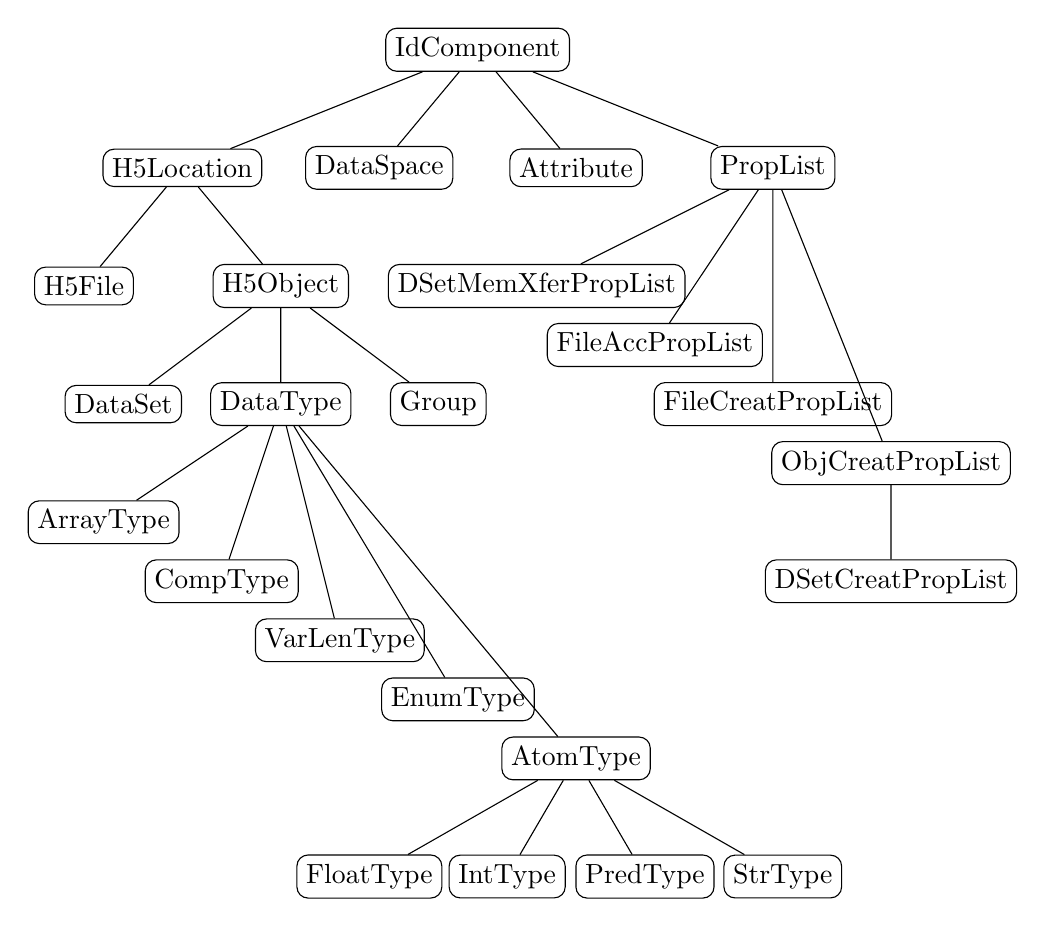
\begin{tikzpicture}[
baseline,
every node/.style = {shape=rectangle, rounded corners, draw, align=center},
]]
  \node {IdComponent}
    child[xshift=-1.5cm]
    {
        node{H5Location}
    	child[xshift=-0.5cm]{node{H5File}}
    	child[xshift=0.5cm]
    		{
    		node{H5Object}
    		child[xshift=-0.5cm]{node{DataSet}}
    		child{
    			node{DataType}
    			child[xshift=0.75cm]{node{ArrayType}}
    			child[xshift=0.75cm,yshift=-0.75cm]{node{CompType}}
    			child[xshift=0.75cm,yshift=-1.5cm]{node{VarLenType}}
    			child[xshift=0.75cm,yshift=-2.25cm]{node{EnumType}}
    			child[xshift=0.75cm,yshift=-3.0cm]
    				{
    				node{AtomType}
    				child[xshift=-0.375cm]{node{FloatType}}
    				child[xshift=-0.125cm]{node{IntType}}
    				child[xshift=0.125cm]{node{PredType}}
    				child[xshift=0.375cm]{node{StrType}} 
    				}
    			}
    		child[xshift=0.5cm]{node{Group}}
    		}
 	}
    child[xshift=-0.5cm]{node{DataSpace}}
    child[xshift=0.5cm]{node{Attribute}}
    child[xshift=1.5cm]{
    	node{PropList}
    	child[xshift=-0.75cm]{node{DSetMemXferPropList}}
    	child[xshift=-0.75cm,yshift=-0.75cm]{node{FileAccPropList}}
    	child[xshift=-0.75cm,yshift=-1.5cm]{node{FileCreatPropList}}
    	child[xshift=-0.75cm,yshift=-2.25cm]{
    		node{ObjCreatPropList}
    		child{node{DSetCreatPropList}}
    		}
    		};
\end{tikzpicture}
}
\caption{Depiction of derivation hierarchy}
\label{graph:hierarchy}
\end{figure}
As stated in the background \ref{seq:background} this project works with \textit{Hagedorn} wavepackets over a fixed time horizon. To make it possible that the simulation can be reproduced or restarted at any given time, the state has to be stored in every time step $\Delta t$. This can be achieved with the classes shown in figure \ref{graph:hierarchy}, where their functionality will be explained from section \ref{seq:internaltypes} to \ref{seq:attribute}.

\section{Internal types and states}
\label{seq:internaltypes}
An interface in general has supported objects and functions. These functions also have preconditions and postconditions whereas objects have valid states. In case of the HDF5 library when these are not fulfilled, an exception is thrown, which could abort or interrupt the program execution. Therefore it is important to always use valid objects and function calls. There are two most common used types. These are \texttt{hsize\_t} and \texttt{H5std\_string}. Variables of type \texttt{hsize\_t} represent native multiple-precision integer and are always used to describe dimensions. This type substitutes the C++ internal \texttt{int} data type. The other is \texttt{H5std\_string} type, which is just an alias for the \texttt{string} data type from the standard library. Furthermore internal valid states are always represented by names using only uppercase letters and with the C prefix for class category as in table \ref{table:corrs}, getrennt with underscore. For example a valid property list state is \texttt{H5P\_DEFAULT}.

\section{H5File}
\label{seq:h5file}
As the name already suggest this class is used to manage the binary file object itself. When a \textit{H5File} is default constructed it further allocates a default \textit{Group} root named "/". To construct a \textit{H5File} a minimal number of two arguments is needed, demonstrated in the code snippet below. The two additional optional arguments are a \textit{FileCreatPropList} and a \textit{FileAccPropList} which would allow further specification. These would be creation and access properties as suggested by the names themselves. In case of this project they are [ueberfluessig] and the \texttt{H5P\_DEFAULT} is sufficient. For the first mandatory argument, which is the filename, a \texttt{H5std\_string} is required. The second one defines the type of creation, which has two valid values. These possible states are \textit{H5F\_ACC\_TRUNC} and \textit{H5F\_ACC\_EXCL}, which are mutually exclusive. The former truncates the file, meaning, if it already exists all data previously stored in the file is erased. The latter fails the construction, if the file already exists under the specified name, which ends up in an thrown exception. It is advised to work with \textit{H5F\_ACC\_TRUNC} because it is simpler and thus errors will less frequently occur.

\begin{lstlisting}
H5File file(string "filename",H5F_ACC_TRUNC);
\end{lstlisting}


\section{Group}
\label{seq:group}
The hierarchy gets implemented through the usage of \textit{Groups}. In case of a \textit{Hagedorn} wavepackets and its corresponding energies the structure in figure \ref{graph:file} is preferred as it corresponds to the structure of the python generated data.

\begin{figure}[ht!]
\centering
\resizebox{\textwidth}{!}{
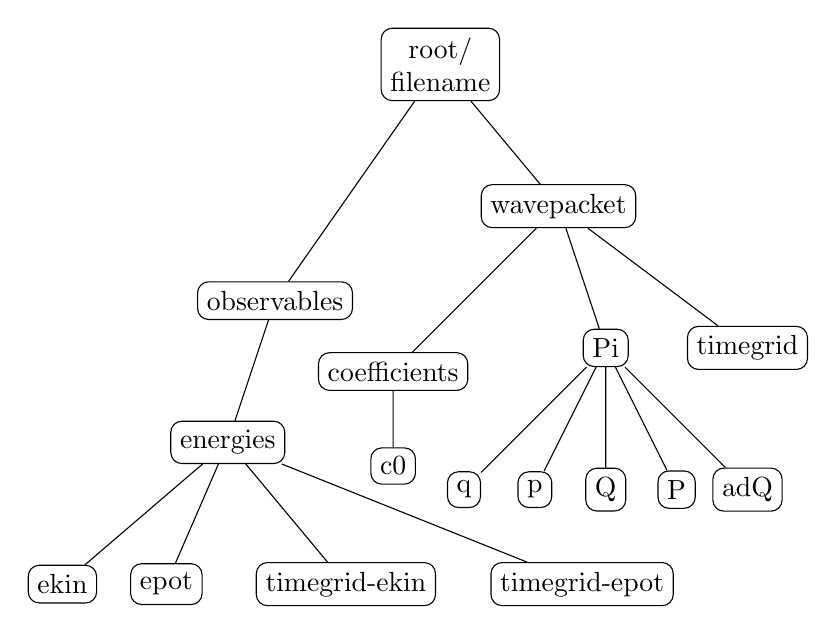
\begin{tikzpicture}[
baseline,
scale=1.2,
every node/.style = {shape=rectangle, rounded corners, draw, align=center},
]]
  \node {root/\\filename}
    child[yshift=-1cm,xshift=-1cm]
    {
    node{observables}
    child[xshift=-0.5cm]
            {
            node{energies}
    		child[xshift=0.5cm]{node{ekin}} 
    		child[xshift=0.1cm]{node{epot}}
    		child[xshift=0.5cm]{node{timegrid-ekin}}
    		child[xshift=1.5cm]{node{timegrid-epot}}
    		} 
    }
    child[xshift=0.5cm] 
    { 
    node {wavepacket}
    child[xshift=-0.25cm,yshift=-0.25cm]{node{coefficients}
    child[yshift=0.5cm]{node{c0}}}
    child[xshift=0.5cm]
    {
    node {Pi}
    child[xshift=1.5cm]{ node {q} }
    child[xshift=0.75cm] { node {p} }
    child { node {Q} }
    child[xshift=-0.75cm] { node {P} }
    child[xshift=-1.5cm] { node {adQ}}    
    }
    child[xshift=0.5cm]{node{timegrid}} 
	};
\end{tikzpicture}
}
\caption{Depiction of desired internal structure of a H5File}
\label{graph:file}
\end{figure}
To create a \textit{Group} only a \texttt{string} argument is required which acts as name but more importantly includes the path. As previously indicated in section \ref{seq:h5file} a textit{H5File} has root \textit{Group} "/" by default after allocation. To accomplish the structure, as shown in figure \ref{graph:file}, the path, beginning at "/", is added to the name. For instance to have a \textit{Group} "wavepacket" after the root "/" and a \textit{Group} "Pi" after "wavepacket" the first name will be modified to "/wavepacket" and the second to "/wavepacket/Pi". This implies that every intermediate node in figure \ref{graph:file} will be a \textit{Group}. The leafs however will be \textit{DataSets} which will be explained in the next section \ref{seq:dataset}. The creating gets invoked from the \textit{H5File} object as the code below shows.

\begin{lstlisting}
file.createGroup(string "grouppath/groupname")
\end{lstlisting}

\section{DataSet}
\label{seq:dataset}
To create a \textit{DataSet} object four arguments are demanded with individual type \textit{string}, \textit{DataType}, \textit{DataSpace} and \textit{DSetCreatPropList}. The first argument, analogous to the \textit{Group}, is the name with its path included. E. g. the \textit{DataSet} "ekin" has the complete name "/observables/energies/ekin". As the name indicates the second and the third argument specify the type and space of the data. Lastly the forth argument defines the desired properties of the \textit{DataSet}. This incorporates which data layout is chosen. The function code is shown below and again invoked by the \textit{H5File}. The \textit{DataSet} has three types of layouts to store raw data. These are \texttt{H5D\_COMPACT}, \texttt{H5D\_CONTIGUOUS} and \texttt{H5D\_CHUNKED}. Figure \ref{fig:datalayout} should illustrate the inner workings of these layouts.

\begin{lstlisting}
file.createDataSet(string "datasetpath/datasetname",DataType type,DataSpace space, DSetCreatPropList list);
\end{lstlisting}

\begin{figure}[ht!]
\resizebox{\textwidth}{!}{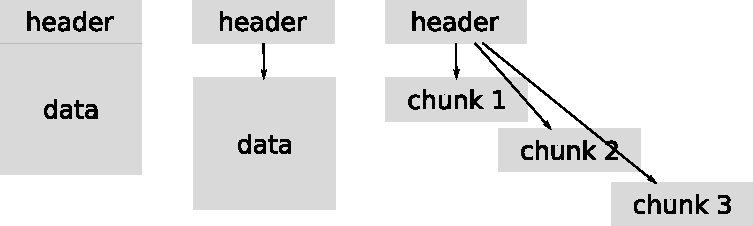
\includegraphics{data_layout.pdf}}
\caption{The three data layouts in \textit{DataSet}}
\label{fig:datalayout}
\end{figure}

If the data is sufficiently small \texttt{H5D\_COMPACT} will be used. In this layout the data address follows right after the header as shown on the left. When the data is larger but still has a constant size, \texttt{H5D\_CONTIGUOUS} in the middle, is the right layout. This one allows that the data to be somewhere arbitrary in memory whereas a link is created into the header. The last layout, \texttt{H5D\_CHUNKED} on the right, is useful assuming the size of the data is unknown. The data will be divided into chunks with the same size where the address of each chunk will be stored in the header. This implies when a chunk is full a new one can be easily allocated and linked in the header, which is ideal for this project. A simulation generates new data in each time step which in essence is ideal for the size of a chunk because it further allows to label each chunk to its corresponding time step. This will be later used to calculate the absolute time point which enables that one can compare chunks of data where the time point is the same.

\section{DataType}
\label{seq:datatype}
The language C++ itself supports data types such as \emph{int}, double, char etc. but these cannot be used directly in a binary data format.
This is caused by the different data representations which are not homogeneous across different operating systems and system architectures. For example the difference between little-endian and big-endian machines. Thus the library has its own definitions which are compatible across platforms which are incorporated into the different classes seen in figure \ref{graph:hierarchy}. It is intuitively clear from their names which classes must be used to describe which data types. For instance for writing floating point numbers the \textit{FloatType} class is used, where it also would be possible to change from IEEE representation to another. In this project the \textit{PredType} and \textit{CompType} are the most relevant classes. From \textit{PredType}, which is predetermined through the C++ language, the \textit{NATIVE\_INT} type is utilized for writing timegrids. The \textit{CompType} class is used for
writing compositions of simple types such as a \textit{struct} of two \textit{doubles}. This is useful to construct a complex data type which will be explained in section \ref{seq:datatypedec}.

\section{DataSpace}
\label{seq:dataspace}
To describe the dimensionality of our data the \textit{DataSpace} class is required. The construction of such a \textit{DataSpace} is straightforward. Firstly the library needs to know the number of dimensions of the desired space. Secondly it has know the number of elements in each dimension. For the second argument an array of \texttt{hsize\_t} is expected instead of \texttt{int} as described in section \ref{seq:internaltypes}. To give the reader an idea the following code depicts the \textit{DataSpace} of a timegrid.

\begin{lstlisting}
int rank = 1;
hsize_t size[rank];
size[0]=number_of_timesteps;
DataSpace limited_timespace(rank,size);
\end{lstlisting}
The problem herein lies in the number of time steps which is known only at runtime. This leads to another approach which is to define a unlimited \textit{DataSpace}. The library allows this if an additional optional argument is added. This argument has to be of the same data type as the second argument and contains the maximum size of each dimension. The library expects that this argument has to be greater or equal than the previous argument otherwise an exception is thrown. For an unlimited space a special state is used namely \texttt{H5S\_UNLIMITED}. The above example code changes to the following if an unlimited space is desired:
\begin{lstlisting}
int rank = 1;
hsize_t size[rank] = {1};
hsize_t maxsize[rank]={H5S_UNLIMITED};
DataSpace unlimited_timespace(rank,size,maxsize);
\end{lstlisting}

\section{PropList}
Most classes require a specific property list at the moment of construction which include additional information. Depending on the object a different property list is needed. All these lists have a common base class namely \textit{PropList} as presented in figure \ref{graph:hierarchy}. The possibilities of these property lists excel the scope of this project easily therefore the default value is enough. The default values are shortly described in table \ref{table:default}.

\begin{figure}[ht!]
\centering
\begin{tabular}{|l|l|}
\hline
Default name value&Influence\\
\hline
\texttt{H5P\_FILE\_CREATE}&\textit{H5FILE} creation\\
\texttt{H5P\_FILE\_ACCESS}&\textit{H5FILE} access\\
\texttt{H5P\_DATASET\_CREATE}&\textit{DataSet} creation\\
\texttt{H5P\_DATASET\_XFER}&raw data transfer\\
\texttt{H5P\_MOUNT}&\textit{H5File} mounting\\
\texttt{H5P\_DEFAULT}&base value for all the above\\
\hline
\end{tabular}
\caption{Table of property list default values and their influence}
\label{table:default}
\end{figure}

Noteworthy for this project is only the \textit{DSetCreatePropList} mentioned in section \ref{seq:dataset} which will be explained in the next section \ref{seq:dscpl}.

\subsection{DSetCreatePropList}
\label{seq:dscpl}
From section \ref{seq:dataset} a \textit{DSetCreatePropList} object is demanded for creating a \textit{DataSet}. As the perceptive reader can guess this property list is used to determine the data layout shown in figure \ref{fig:datalayout}. The property list is responsible for setting the layout to \texttt{H5D\_COMPACT}. This is important because only data with this layout can be dynamically extended later on during a simulation. 
\begin{lstlisting}
//create default H5P_DATASET_CREATE
DSetCreatePropList list;
//set chunked data layout
list.setChunk(int number_of_dim,hsize_t* dim);
//setting the fill value after allocation
list.setFillValue(DataType type,void* default_value);
\end{lstlisting}
The above code achieves to set chunked layout into the property list for the construction of a \textit{DataSet}. Furthermore a default fill value can be defined which is utilized to fill new allocated memory.

\section{Attribute}
\label{seq:attribute}
Additionally to writing data in binary format it should also incorporate saving corresponding meta data. This can be easily done with \textit{Attributes} which must be attached to an affiliated \textit{Group} or \textit{DataSet}. The allocation of such an \textit{Attribute} is similar to a \textit{DataSet} meaning a \textit{DataType} and \textit{DataSpace} is also demanded. For its property list only the \texttt{H5P\_DEFAULT} is allowed which the library enforces otherwise an exception is thrown. For illustration see the subsequent code.
\begin{lstlisting}
Attribute attribute;
//group attribute
attribute = group.createAttribute(string "attributename",DataType type,DataSpace space,PropList plist);
//dataset attribute
attribute = dataset.createAttribute(string "attributename",DataType type,DataSpace space,PropList plist);
\end{lstlisting}

\chapter{Writer Template}
\section{Link to Eigen library}
\label{seq:linkeigen}
As mentioned in background \ref{seq:background} the simulation boils down to propagating the set \{q,p,Q,P,S\}, where q and p are $D$ dimensional real-valued vectors, Q and P complex $D \times D$ matrices and S the global complex phase. A possible interface to manage these matrices and vectors is the \textit{Eigen} library. The definition of an \textit{Eigen} matrix has the following form:
\begin{lstlisting}
Eigen::Matrix<complex<double>,row_dim,column_dim> mat;
\end{lstlisting}
Note that this is a class template over three parameters namely type, row-dimension and column-dimension. Therefore the overall implementation will also be a template. In the current version only scalar \textit{Hagedorn} wavepackets are supported thus only one dimension parameter $D$ is utilized but the framework can still easily be extended in further works. As discussed in section \ref{seq:datatype} normal types are not writable, hence the type is defined through the library. This declared type is not necessarily the same as the template argument from \textit{Eigen}, but is still similar enough to permit basic transformation functions which are discussed in section \ref{seq:transform}.

\section{DataType Declaration}
\label{seq:datatypedec}
In this context simulation means manipulating complex numbers. To build a \textit{DataType} the library needs access to its members thus the standard \texttt{complex} class cannot be utilized. Therefore a \texttt{struct} is most suitable for defining the fundamental structure since all its members are by default public accessible. Hence the declaration of complex numbers looks like this:
\begin{lstlisting}
struct ctype
{
  double real;
  double imag;
} instance_of_ctype;
\end{lstlisting}
This can now be used by the library to create the corresponding \textit{DataType} which in this case the \textit{CompType} is most suitable because \texttt{ctype} is a composition of simple data types. To be compatible with python the same labels for its members have to be used which result in the following code:
\begin{lstlisting}
CompType hdfctype_(sizeof(instance_of_ctype));
hdfctype_.insertMember("r",HOFFSET(ctype,real), PredType::NATIVE_DOUBLE);
hdfctype_.insertMember("i",HOFFSET(ctype,imag), PredType::NATIVE_DOUBLE);
\end{lstlisting}
Worth noting is that the constructor of \textit{CompType} relies on the \texttt{sizeof} operator which tells how many bytes for an instance of this type is needed. The string labels "r" and "i" are utilized for the real respective the imaginary part of a complex number. \texttt{HOFFSET} is a simple function which returns at which position counted in bytes the second argument is located in the first argument. In this case the first \texttt{double}(real) is located at "0" and the the second one(imag) at "8" since one \texttt{double} is $8$Byte long. Finally the last argument is the type inserted at this position. Since already discussed in section \ref{seq:datatype} \texttt{double} cannot be used directly but the library provides these definitions through the \textit{PredType} class. The members of \textit{PredType} are constant and are fixed through the C++ language itself.\\

\section{Constructor}
\label{seq:ctor}
Since the data type declaration only has to be initialized once, it is suitable to pack it into the constructor of this writer template. The constructor only expects one string argument, namely the filename. Therefore the the constructor can be written accordingly:
\begin{lstlisting}
template<int D>
...
//ctor
hdf5writer(string name):filename_(name), hdfctype_(sizeof(instanceof)),file_(filename_,H5F_ACC_TRUNC)
{
	hdfctype_.insertMember("r",HOFFSET(ctype,real), PredType::NATIVE_DOUBLE);
	hdfctype_.insertMember("i",HOFFSET(ctype,imag), PredType::NATIVE_DOUBLE);
}
\end{lstlisting}
Observe that there are two implicit constructor calls after instantiation of the filename. For the former refer to section \ref{seq:datatypedec} whereas for the latter see section \ref{seq:h5file}.

\section{Write options}
To enable customization about what and when something is written an additional layer was inserted. This was done with functions which set the desired configuration. In the current implementation there are three choices to make. By default writing \textit{Hagedorn} wavepackets is enabled, whereas writing the corresponding norm and the energies are disabled. This behavior is directed by a boolean. As already mentioned in section \ref{seq:dataset} for each chunk written also a time label is attached. This was achieved by writing for each important \textit{DataSet} an additional \textit{DataSet} at the same level with the same length, where each entry is an \texttt{int}, symbolizing the number of time steps passed since the beginning of the simulation. These are shown in figure \ref{graph:file} where "timegrid" was used in its name. The corresponding customization thereof is to set the difference between two consecutive entries. More precisely, it is the choice if a \textit{DataSet} should be written in each time step($d=1$) or every second time step($d=2$) etc. The supported functions are listed subsequently:
\begin{lstlisting}
set_write_packet(true|false);
set_write_norm(true|false);
set_write_energies(true|false);
set_timestep_packet(1|2|3|...);
set_timestep_norm(1|2|3|...);
set_timestep_energies(1|2|3|...);
set_timestep_ekin(1|2|3|...);
set_timestep_epot(1|2|3|...);
\end{lstlisting}

\section{DataSet paths}
The structure in figure \ref{graph:file} is fixed in the implementation as it is analogous to the python generated data. Furthermore the names of all \textit{Groups} and \textit{DataSets} are also already determined. The data test is build on these as well. This can be problematic, once a change happens in the python or C++ implementation, where the structure is affected. Luckily the library throws an invalid path exception if such a change occurs where the paths are no longer valid. Future work could include to make data test path independent for \textit{DataSets}.

\section{Prestructure}
\label{seq:prestructure}
This function is a bundle of steps which either have to be done prior or are constant during the writing process. The function definition is shown subsequently:
\begin{lstlisting}
template<class MultiIndex>
prestructuring(ScalarHaWp<D,MultiIndex> packet,double dt);
\end{lstlisting}
The dimension $D$ and the class \texttt{MultiIndex} are prerequisite for constructing a scalar \textit{Hagedorn} wavepacket and are detailed explained in the thesis of Michaja B\"osch \cite{bt_michajab}. A scalar \textit{Hagedorn} wavepacket includes a matrix of coefficients and the set \{q,p,Q,P,S\}. The coefficient dimension is dependent on $D$ and \texttt{MultiIndex}, therefore the number of coefficients is calculated and stored first in this function. Next the \textit{Groups} of figure \ref{graph:file} is set. Additionally some \textit{Attributes} are attached to the root group such as the time step $dt$. As discussed in section \ref{seq:dataset} each \textit{DataSet} has to be chunked according to a time step. Hence this chunk dimension is set in the next step for all \textit{DataSets} specified in the write options. E.g. for a packet the chunk-dimension for the coefficients, q, p, Q, P, and S have to be set into an instance of \textit{DSetCreatPropList} individually. 
For instance a chunk-dimension of $2 \times 2$ matrix in time is declared in the following form:
\begin{lstlisting}
hsize_t chunk[3] = {1,2,2};//{time_dim,row_dim,column_dim}
\end{lstlisting}
For further instruction see section \ref{seq:dscpl}. Before it is possible to allocate all \textit{DataSets} according to figure \ref{graph:file} also individual \textit{DataSpaces} have to be declared. Luckily it is possible to reuse all chunk-arrays as arguments for their own \textit{DataSpace} with the additional array argument according to section \ref{seq:dataspace}. Now all building blocks are ready to allocate in the next step all \textit{DataSets}. It can be observed that there is a source and destination \textit{DataSpace} with a corresponding selection in each time step. The destination \textit{DataSpace} grows over time within the file and thus is not constant. Different from the destination, the source \textit{DataSpace} and its selection is constant and therefore can be fixed in this step for the whole simulation. Notice that \textit{DataSpace} is the space of possible positions where data can be written to, whereas it needs to be specified which elements in \textit{DataSpace} are utilized. This is done with a selection which is described by a hyperslab and will be explained in the next section \ref{seq:selection}.

\section{Selection}
\label{seq:selection}
As already mentioned in the previous section \ref{seq:prestructure} a selection within a \textit{DataSpace} is represented with a hyperslab. A hyperslab consists of four arrays namely:
\begin{lstlisting}
hsize_t start[3] = {time_label,1,1};
hsize_t count[3] = {time_label,3,2};
hsize_t block[3] = {time_label,1,1};
hsize_t stride[3] = {time_label,2,2};
\end{lstlisting}
Notice that the first dimension is always reserved for the time dimension. The implementation has an internal index for storing the current simulation step which is used as the label. Thus only the index for the next time step has to be incremented without altering the code for the selection. The following figure \ref{fig:hyperslab} illustrates why four arrays are required to represent a hyperslab.

\begin{figure}[ht!]
\centering
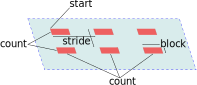
\includegraphics[scale=1.8]{selection.pdf}
\caption{hyper-slab illustration}
\label{fig:hyperslab}
\end{figure}
In figure \ref{fig:hyperslab} the blue plane symbolizes a matrix in three dimension. The first dimension is reserved for time meaning the blue plane depicts a matrix at some fixed time point. One red block represents one element in this matrix. Thus this figure displays the hyperslab from the previous code segment. The selection is done by the \textit{DataSpace} itself whereas the \texttt{H5S\_SELECT\_SET} argument is recommended to overwrite the old selection.
\begin{lstlisting}
dataspace.selectHyperslab(H5S_SELECT_SET, count, start, stride, block);
\end{lstlisting}
In case that a continuous block of data is written the last two arguments can be omitted.
\begin{lstlisting}
dataspace.selectHyperslab(H5S_SELECT_SET, count, start);
\end{lstlisting}


\section{Transformation}
\label{seq:transform}
As indicated in section \ref{seq:linkeigen} basic transformations is applied to the \textit{Eigen} matrices. The internal data in a \textit{Eigen} matrix can be extracted with the \texttt{matrix.data()} function. Either the data is of type \texttt{complex<double>} or \texttt{double} which can be transfered to \texttt{ctype}. From \texttt{complex<double>} its members can be simply copied over whereas for a \textit{double} the imaginary part is simply set to zero. After this step all data originally saved in a \textit{Eigen} matrix are now stored in vectors of \texttt{ctype}. Later on the data is again extracted with \texttt{vector.data()} function and passed on to HDF library for writing. The reason for this transformation from \texttt{complex<double>} or \texttt{double} to \texttt{ctype} is that in the writing function call \texttt{hdfctype\_} will be used as type argument. Since \texttt{hdfctype\_} is constructed from \texttt{ctype}, see section \ref{seq:ctor}, it can be safely assumed that the library can write pointers of type \texttt{ctype}.

\section{Writing}
\label{seq:writing}
All tools are ready to look at the actual writing function call for \textit{DataSets} and \textit{Attributes}:
 
\begin{lstlisting}
dataset.write(void* src,DataType type,DataSpace srcspace,DataSpace dstspace);
attribute.write(DataType type,void* src);
\end{lstlisting}
Notable is that the size of \texttt{src} is hidden in the selection of \texttt{srcspace}. Furthermore the destination is implicit given by the \texttt{datasetname} where the function call occurred. When the selection of \texttt{srcspace} and \texttt{dstspace} does not match in size an exception is thrown. There are only two types used as \textit{DataType}. For actual data \texttt{hdfctype\_} is utilized and \texttt{PredType::NATIVE\_INT} for timegrids. Remember also that all \texttt{srcspaces} are constant and therefore set in section \ref{seq:prestructure}.

\section{Extension}
\label{seq:extension}
The \textit{DataSets} in section \ref{seq:dataset} were explicitly constructed such that they have a chunked memory layout. This is useful now because the library can only extend this type of layout with the succeeding function call: 
\begin{lstlisting}
dataset.extend(hsize_t* dimension);
\end{lstlisting}
The new dimension is as expected an array of \texttt{hsize\_t} where there are two effects. When an entry in the array is smaller than the \textit{DataSet} itself, it will get shrunk along this direction. Alternatively if an entry is larger than the \textit{DataSet} itself, it will get extended along this direction. There will be no effect in case the argument is of the same size as the \textit{DataSet} itself. It is obvious that the \textit{DataSets} in this project only grow in the direction of time per construction. Thereby the chunk dimension can be reused except for the first(time) entry. For this entry an index for each individual \textit{DataSet} is utilized to keep track of the current size. Bear in mind that this index is not the same as the current time index which is used to write timegrids.

\section{Update}
\label{seq:update}
Naturally since all \textit{DataSets} were extended the corresponding \textit{DataSpace} used as the destination is outdated. Furthermore each individual index used to keep track of the number of chunks used in section \ref{seq:extension} has to be incremented. Conveniently the library provides a function to extract the \textit{DataSpace} from a \textit{DataSet} namely:
\begin{lstlisting}
DataSpace newdataspace = dataset.getSpace();
\end{lstlisting}
Now all outdated \textit{DataSpaces} are updated with the help of the extended \textit{DataSets}. This function also represent the last action done in the current time step. All actions from \ref{seq:selection} to \ref{seq:update} are repeated in each time step of the simulation. Remember the transformation is included because in each time step the \textit{Hagedorn} wavepacket is propagated according to the chosen scheme and thus was modified.

\section{Poststructure}
\label{seq:poststructure}
After the time loop of the simulation it is important to finalize all structures from the library. Furthermore the last extension has to be reversed since no new data will be written. This is easily done with the same function but with a smaller index as explained before in \ref{seq:update}. All variables allocated on the stack are deleted automatically by the operating system and thus can be neglected. The others allocated with the \texttt{new} operator should be freed manually. Sensibly in this project all these pointer objects are forwarded to the standard library through \texttt{shared\_ptr} container. Likewise \texttt{vector} is managed also by the standard library and thus the library guarantees that these objects will be freed correctly. To use the standard library for all objects is always a good approach because it can prevent data corruption or data loss.

\section{Simulation in a picture}
The functionality of this writer template can be easily visualized when only one \textit{DataSet} is considered, see figure \ref{fig:illustration}.
\begin{figure}[ht!]
\resizebox{\textwidth}{!}{
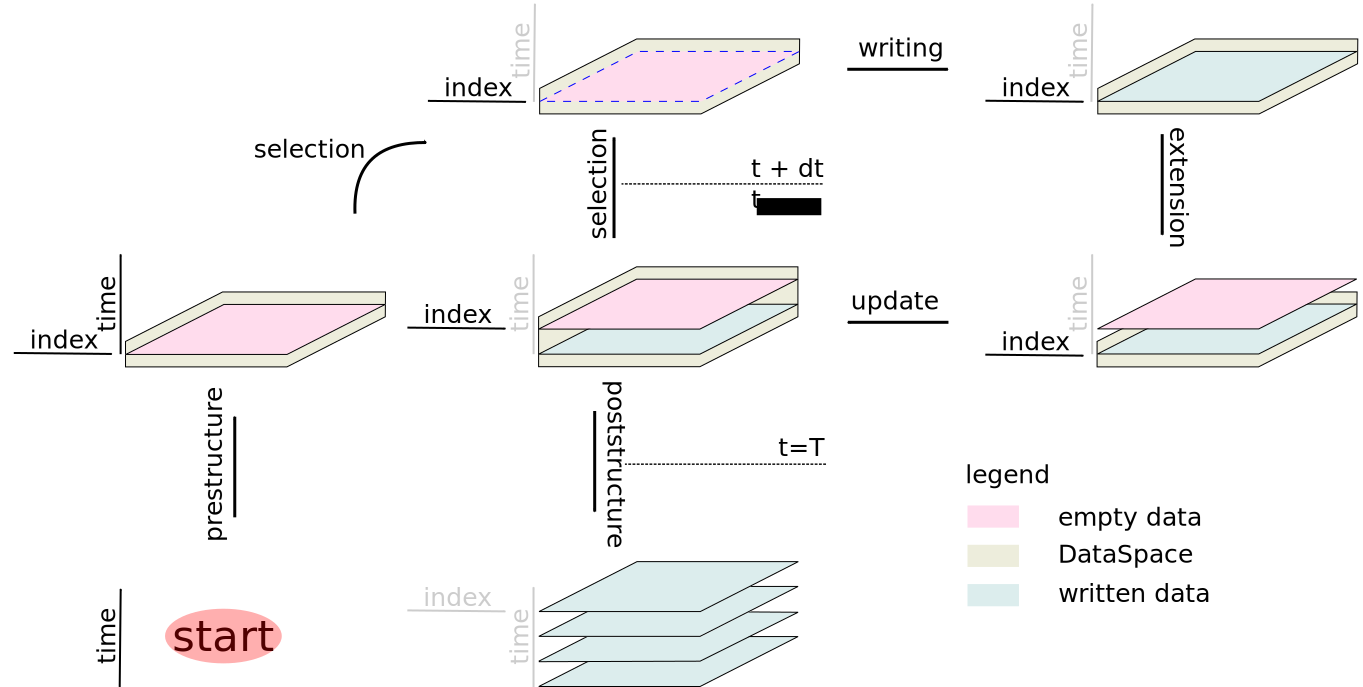
\includegraphics[scale=1.0]{writing_dataset.pdf}
}
\caption{Illustration of inner workings for a \textit{DataSet} in the simulation}
\label{fig:illustration}
\end{figure}
The start symbolizes the constructor of this class. The cycle begins with the selection process which sets a hyperslab, indicated by the blue dashed line. The section \ref{seq:selection} through \ref{seq:update} are element of this cycle which halts only when the time step arrived at $T$. Then the simulation gets finished with the function \ref{seq:poststructure}.

\section{Usage in Simulation}
The following code snippet shows the key functionality to use this class for writing \textit{Hagedorn} wavepackets:

\begin{lstlisting}
//Simulation settings
...
io::hdf5writer<D> writer("simulation_filename.hdf5");

writer.prestructuring<MultiIndex>(packet,dt);

//Time loop(propagation)
for(real_t t = 0; t < T; t += dt)
{
	//Write wavepacket
	writer.store_norm(packet);
	
	//Propagate wavepacket
   	propagator.propagate(packet,dt,V);
}

writer.poststructuring();
\end{lstlisting}
A more detailed version can be found in the appendix. How to generate the mandatory settings indicated with \texttt{...}, it is advised to consult the preceding works found in \cite{bt_michajab}, \cite{st_benedekv} and \cite{bt_lionelm}. Additionally most information can be found in the documentation of the C++ implementation \cite{libwaveblocks}.

\chapter{Data Test}

\section{Introduction to GoogleTest}
There are two main ways to test objects with \textit{GoogleTest}. For the interested reader a more detailed description can be found in the git repository \cite{googletestdoc}, where the Primer.md and AdvancedGuide.md examples are strongly suggested. Of importance is to define a test class for reusing certain objects for all tests. These objects in this case are the two \textit{H5Files}, the \textit{DataType} used in the writing process and the \textit{Attributes} saved in the root group of the two files. One of these \textit{Attributes} is the time step $\Delta t$ utilized for the data matching. When there are two files in general they do not have necessarily the same time step size. However, mapped with the corresponding timegrid, some of the data match to the same timepoint, and therefore can be compared. This is carried out by a function at the beginning, which tests if two \textit{DataSets} have matching timepoints, which will be stored into a list. If the list is empty a message will be printed and the program continues with the next \textit{DataSet}.

\section{The Main File}
\label{seq:testmain}
The main file consists of the test class for the shared objects, all test fissures which are based on the test class and the main function which invokes the test itself. The subsequent code snipped shows the core base structure described before:

\begin{lstlisting}
#include "gtest/gtest.h"
int global_argc;
char** global_argv;
#define abstol 1e-6
...

class TestHDF : public ::testing::Test
{
	protected:
	TestHDF();
	virtual ~TestHDF();
	void SetUp();
	void TearDown();
	void time_matching(...);
	
	struct ctype{...};
	H5File cppfile;
	H5File pyfile;
	CompType hdfctype_;
	double dt_cpp;
	double dt_py;
	...
};

TEST_F(TestHDF,Testpacket)
{...}
TEST_F(TestHDF,Testenergies)
{...}
TEST_F(TestHDF,Testnorm)
{...}

int main(int argc,char* argv[])
{
	global_argc=argc;
	global_argv=argv;
	::testing::InitGoogleTest(&argc,argv);
	return RUN_ALL_TESTS();
}
\end{lstlisting}
First the \textit{TestHDF} class gets constructed where we use global argc and argv arguments to transfer the filenames from the console to the class. Notice also that \textit{TestHDF} needs to derive from \texttt{::testing::Test} from \textit{GoogleTest} to work. Then in the main function the test fissures are invoked with the \texttt{RUN\_ALL\_TESTS()} call. For a test fissure \texttt{TEST\_F()} an additional \texttt{SetUp()} function is provided for further specifying test settings. Afterwards each test fissure also gets cleaned up with the \texttt{TearDown()} function. In the test fissure itself the data test takes place. First the time matching function is invoked with the timegrids of both files as arguments. If the prepared list is not empty than the correct values are loaded from the \textit{H5Files}. These values are then compared with \texttt{EXPECT\_NEAR(...)} function provided by the test framework which compares the difference of two \textit{doubles} to an absolute tolerance. This process will be repeated for each matching \textit{DataSet} in these two files until \texttt{RUN\_ALL\_TESTS()} returns $1$ which indicates successful termination. If the difference between two \textit{doubles} is larger than the defined absolute tolerance they will be printed out automatically and the test will proceed anyway.

\chapter{Conclusion}
This project enabled easy data testing between the current python and C++ implementation which propagate scalar \textit{Hagedorn} wavepackets. It is no longer dependent on the external project \cite{eigen3-hdf5} and does no longer derive types from \textit{Eigen} matrices. The writing type and the hierarchy is fixed throughout but compatible with the current python implementation. At this moment only scalar \textit{Hagedorn} wavepackets can be written and tested but the template can easily be extended.

\section{Further Work}
